
\documentclass{article}
 \usepackage{graphicx}
\setlength{\parindent}{0em}
\setlength{\parskip}{1em}
\title{Proof of Concept - Elaboration}
\author{Osmond Chiu}


\begin{document}
\maketitle
\section*{Planned Thesis Topic}

My planned thesis research will be inductive research that aims to understand re-nationalisations in Australia. Re-nationalisations are when privatised government functions are brought back under public ownership.\par
The aim is to work out why these re-nationalisations occurred through compiling a list of re-nationalisations to identify common factors and examining key case studies.

\section*{Computational Analysis}
\subsection*{Decomposing}
There are a range of discrete tasks for this job. It will involve breaking down into:
\begin{itemize}
    \item defining what data needs to be collected
    \item determining the available resources to conduct the research
    \item conducting the research
    \item collecting the data
    \item organising the collected data
    \item analysing the collected data
    \item determining if the process needs to be repeated
\end{itemize}

\subsection*{Pattern Recognition}
There will be some recurring patterns in how I organise the collected data including metadata and tagging sources.\par

\subsection*{Algorithm}
Step-by-step, this job would likely involve:
\begin{enumerate}
\item Defining the research aim
\item Determining parameters such as time period, location and keywords for research
\item Identifying available sources and databases
\item Researching what tools interact with those sources and databases
\item Testing the tools
\item Using the tool, if it works
\item Saving sources
\item Producing metadata
\item Organising sources
\item Analysing sources
\item Deciding if the process needs to be repeated because the research aim is not met
\end{enumerate}

\section*{Elaboration}

There are a range of technologies that could help deliver the step-by-step requirements listed in my algorithm.

\subsection*{Requirements}

Of the steps outlined, the following steps could be improved with tools:
\begin{itemize}
\item Using the tool to interact with sources and databases
\item organising saved sources.
\item analysing sources 
\end{itemize}\par

The requirement for the first step are tools that can conduct a search for different keywords in documents as the term "re-nationalisation" is not always used. The sources are most likely to primarily be newspaper articles.\par
\par
Requirements for organising sources might be a tool to tag and keep notes for each source Without having to re-read sources, enabling a de facto annotated bibliography.
\par
Analysing sources would require being able to do a text analysis of sources to determine what keywords are used and whether there are any patterns that can be identified across multiple sources about re-nationalisation.
\par

\subsection*{Data Collection}
\subsubsection*{Delivery}

The first requirement can be met by using a tool to capture newspaper articles about examples of re-nationalisation in Australia from online archives.\par

The use of Application Programming Interfaces to conduct searches within aggregators may be the best way to deliver that requirement. An API that could conduct searches on Factiva and ProQuest Australia and New Zealand Newsstream, narrowed to specific keywords in text and Australian newspaper sources.\par

It may require writing some custom script to use the APIs to capture sources, export them and associated metadata.\par 

\subsubsection*{Mitigating risks}

There are risks with data collection, for example, it is not immediately clear that some resources can use APIs such as Google Scholar. Identifying what resources have APIs that may be useful should be done first to know how much work must be done. Time may be wasted on tools to run scripts when there are no APIs.\par

There may be other difficulties automating. Terms and Conditions of ProQuest and Factiva, which is what would be useful for more recent newspaper articles states that users shall not text mine or data mine. This information is at \begin{verbatim}https://libguides.mq.edu.au/textdatamining/publisher_resources\end{verbatim}

Finally, the risk may be that the tool does not find much information meaning it may have been a waste of time.\par

\subsubsection*{Result of Test}

I examined and was not able to locate any APIs for the news aggregators. Advice provided indicated that ProQuest and Factiva do not have freely accessible APIs and would charge for their usage.

Manual searches using aggregators such as ProQuest, Factiva and Google Search. It will be necessary to keep track of search terms used by producing metadata.

\subsection*{Text Analysis}
\subsubsection*{Delivery}

The third requirement may be met through using a text analysis tool to analyse and visualise data. It would first require collecting sources to feed into the tools.\par  

\subsubsection*{Mitigating risks}

With difficulties in automating data collection, analysing the data may be an alternative. There are open source tool to conduct an open source, textual analysis such as Voyant.

The big risk may be that the tool does not produce any useful output from the included information meaning it may have been a waste of time. Testing it beforehand and understanding what kind of output may be generated will therefore be important. Examining the help documentation will assist, which is available at https://voyant-tools.org/docs/\par

\subsubsection*{Result of test}

I tested the tool by uploading a three articles on the reversal of the privatisation of the Port Macquarie Base Hospital to Voyant.

\begin{figure}[htp]
    \centering
    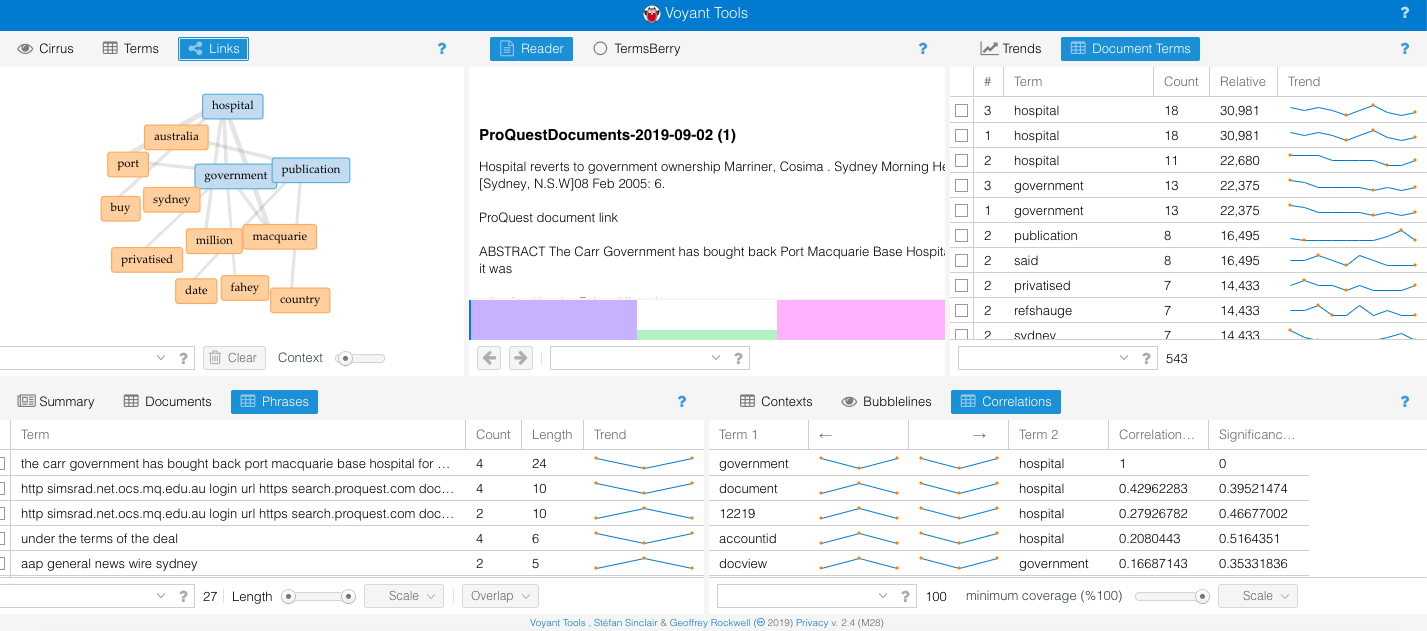
\includegraphics[width=10cm]{Voyant.png}
    \label{fig:voyant}
\end{figure}

The results highlighted the frequency of terms such as 'public', 'government' and 'privatised'. Given the language used and the number of sources, it seems unlikely to provide any useful analysis about why re-nationalisation occurred without understanding the context.

\subsection*{Organising Data}
\subsubsection*{Delivery}

The second requirement could be met by using a software that could organise, collect and keep information on sources. Ideally it would be able to tag themes, locate key terms, include notes and enable examining across multiple sources. There are a range of options including Zotero, NVivo or Hypothes.is that could be explored.

NVivo has more functions but is not an open source tool meaning it may change or cost significant. Hypothes.is is an annotation wheras Zotero is bibliographical software

Ambar has a tagging and search capability but will require a small payment or some script to be installed. An explanation is provided.

Open Semantic Desktop has a wider range of capabilities, tagging with full text search, exploratory search, analytics and text mining in many documents

\subsubsection*{Mitigating risks}

A key risk is not all tools having the same features. An incorrect choice could lead to a problem whereby a feature is not available, resulting in more work. It may be a case where more than one tool will need to be used. For example, Open Semantic Search has most features but not does appear to be a good referene manager for a thesis.\par 

It will be important to search for information comparing the features of different software and test the software for likely needs such as organising, tagging, citations, annotating sources.\par

\subsubsection*{Result of test}

Open Semantic as it had the most features covered off (tagging, search, text analysis)

Identify if there is a bibliography or referencing feature

Zotero


\subsection*{Conclusion}

My elaboration has identified that improving the organisation of data is where tools could aid the most.

While data collection will need to be done manually, a combination of Open Semantic and Zotero can be used to improve the organisation of data. There are other tools but they




\end{document}